\chapter{Experiments}\label{r:experiments}

This chapter presents a comprehensive experimental evaluation of proposed \method{} framework for generating \framework{}. This work systematically evaluates the method's ability to generate diverse, high-quality samples while maintaining invariant set membership across three complementary experimental paradigms: individual neuron activation analysis, sparse autoencoder (SAE) feature investigation, and classifier output preservation.

\section{Experimental Design}

The experimental evaluation addresses the following core research questions:
\begin{enumerate}
\item Can \method{} generate visually diverse samples that maintain identical activation patterns for interpretable neurons?
\item Do generated samples reveal semantic patterns beyond those present in typical training data?
\item How effectively does the method preserve complex feature representations learned by sparse autoencoders?
\item Can the framework maintain classifier predictions while generating semantically meaningful variations?
\end{enumerate}

\subsection{Infrastructure and Implementation}

All experiments were conducted on NVIDIA A100 GPUs (1-4 units) using PyTorch. This work employs LightningDiT as proposed diffusion backbone with SGD optimization at learning rate $\eta = 10$ based on empirical hyperparameter evaluation (see \cref{appendix:hyperparameters}). Each experimental condition generates 32-256 samples due to computational constraints, representing a balance between statistical validity and resource efficiency.

\subsection{Evaluation Framework}

This work employs a multi-faceted evaluation approach combining quantitative precision metrics with qualitative semantic analysis:

\textbf{Quantitative Metrics:}
\begin{itemize}
\item \textbf{Activation Fidelity}: $L_1$ and $L_2$ norm deviations from target values
\item \textbf{Probability Preservation}: Kullback-Leibler (KL) divergence for probability distributions, defined as
\begin{equation}
D_{KL}(P \parallel Q) = \sum_{x} P(x) \log \frac{P(x)}{Q(x)}
\end{equation}
where $P(x)$ represents the target probability distribution and $Q(x)$ the generated distribution
\item \textbf{Spectral Coherence}: Frequency domain analysis using ideal low-pass filters (see \cref{appendix:spectral_analysis})
\item \textbf{Image Quality}: Fréchet Inception Distance (FID) relative to natural image statistics
\end{itemize}

\textbf{Qualitative Assessment:}
\begin{itemize}
\item Semantic diversity within invariant sets
\item Visual coherence and absence of adversarial artifacts
\item Alignment between generated patterns and expected neuron/feature selectivity
\end{itemize}

\section{Individual Neuron Activation Analysis}

Building upon mechanistic interpretability advances, this work targets neurons with well-characterized semantic properties identified through the Semantic Lens framework \citep{dreyer2025mechanisticunderstandingvalidationlarge}. This analysis investigates whether \method{} can generate diverse visual patterns that consistently activate specific semantic detectors.

\subsection{Target Neuron Selection}

The three neurons were selected from ResNet50's final feature layer based on high semantic alignment scores and interpretable activation patterns:

\begin{itemize}
\item \textbf{Neuron \#1656 (Zebra Striping)}: Alignment score $r = 0.945$, responds to black-white striped patterns
\item \textbf{Neuron \#1052 (Honeycomb Structure)}: Alignment score $r = 0.880$, activates on hexagonal cellular structures  
\item \textbf{Neuron \#421 (Gyromitra Morphology)}: Alignment score $r = 0.952$, responds to convoluted, brain-like surface textures
\end{itemize}

\subsection{Experimental Protocol}

For each target neuron $n$, the following protocol was followed:
\begin{enumerate}
\item Select a query image $\mathbf{x^*}$ that strongly activates the neuron
\item Define the invariant set constraint: $n(\mathbf{x}) = n(\mathbf{x^*})$
\item Apply \method{} to generate 32 samples maintaining this constraint
\item Evaluate activation fidelity, visual quality, and semantic diversity
\end{enumerate}

\subsection{Quantitative Results}

\begin{figure}[h]
\centering
\includegraphics[width=\linewidth]{figures/main/sae_results_2.png}
\caption{ \textbf{C} - Original and Generated logits comparison  \textbf{1}: \#1656 (Zebra Striping), \textbf{2}: \#1052 (Honeycomb), \textbf{3}: \#421 (Gyromitra). \textbf{D} - top logit activation in target neuron. There are 49 logits in target neuron of last convolution layer in ResNet50 model}
\label{fig:experiment_1_1}
\end{figure}

Table~\ref{tab:neuron_results} presents quantitative evaluation metrics across target neurons. The consistently low $L_2$ losses (< 1.0 on unbounded logits) demonstrate precise activation preservation, while FID scores indicate maintenance of natural image statistics.

\begin{table}[h!]
\centering
\begin{tabular}{lcccc}
\toprule
\textbf{Neuron} & \textbf{Concept} & \textbf{$L_2$ Loss} & \textbf{FID Score}\\
\midrule
\#1656 & Zebra Striping & 0.59 $\pm$ 0.12 & 7.91 \\
\#1052 & Honeycomb & 0.87 $\pm$ 0.16 & 8.04\\
\#421 & Gyromitra & 0.32 $\pm$ 0.05 & 8.07\\
\midrule
\textbf{Average} & -- & \textbf{0.59 $\pm$ 0.11} & \textbf{8.06}  \\
\bottomrule
\end{tabular}
\caption{Quantitative evaluation results for individual neuron activation analysis. $L_2$ losses computed on unbounded activation logits; values < 1.0 indicate excellent preservation. FID scores computed against Imagenet-1k  image statistics. Results averaged over 32 generated samples per neuron.}
\label{tab:neuron_results}
\end{table}

\subsection{Qualitative Analysis}

\begin{figure}[h]
\centering
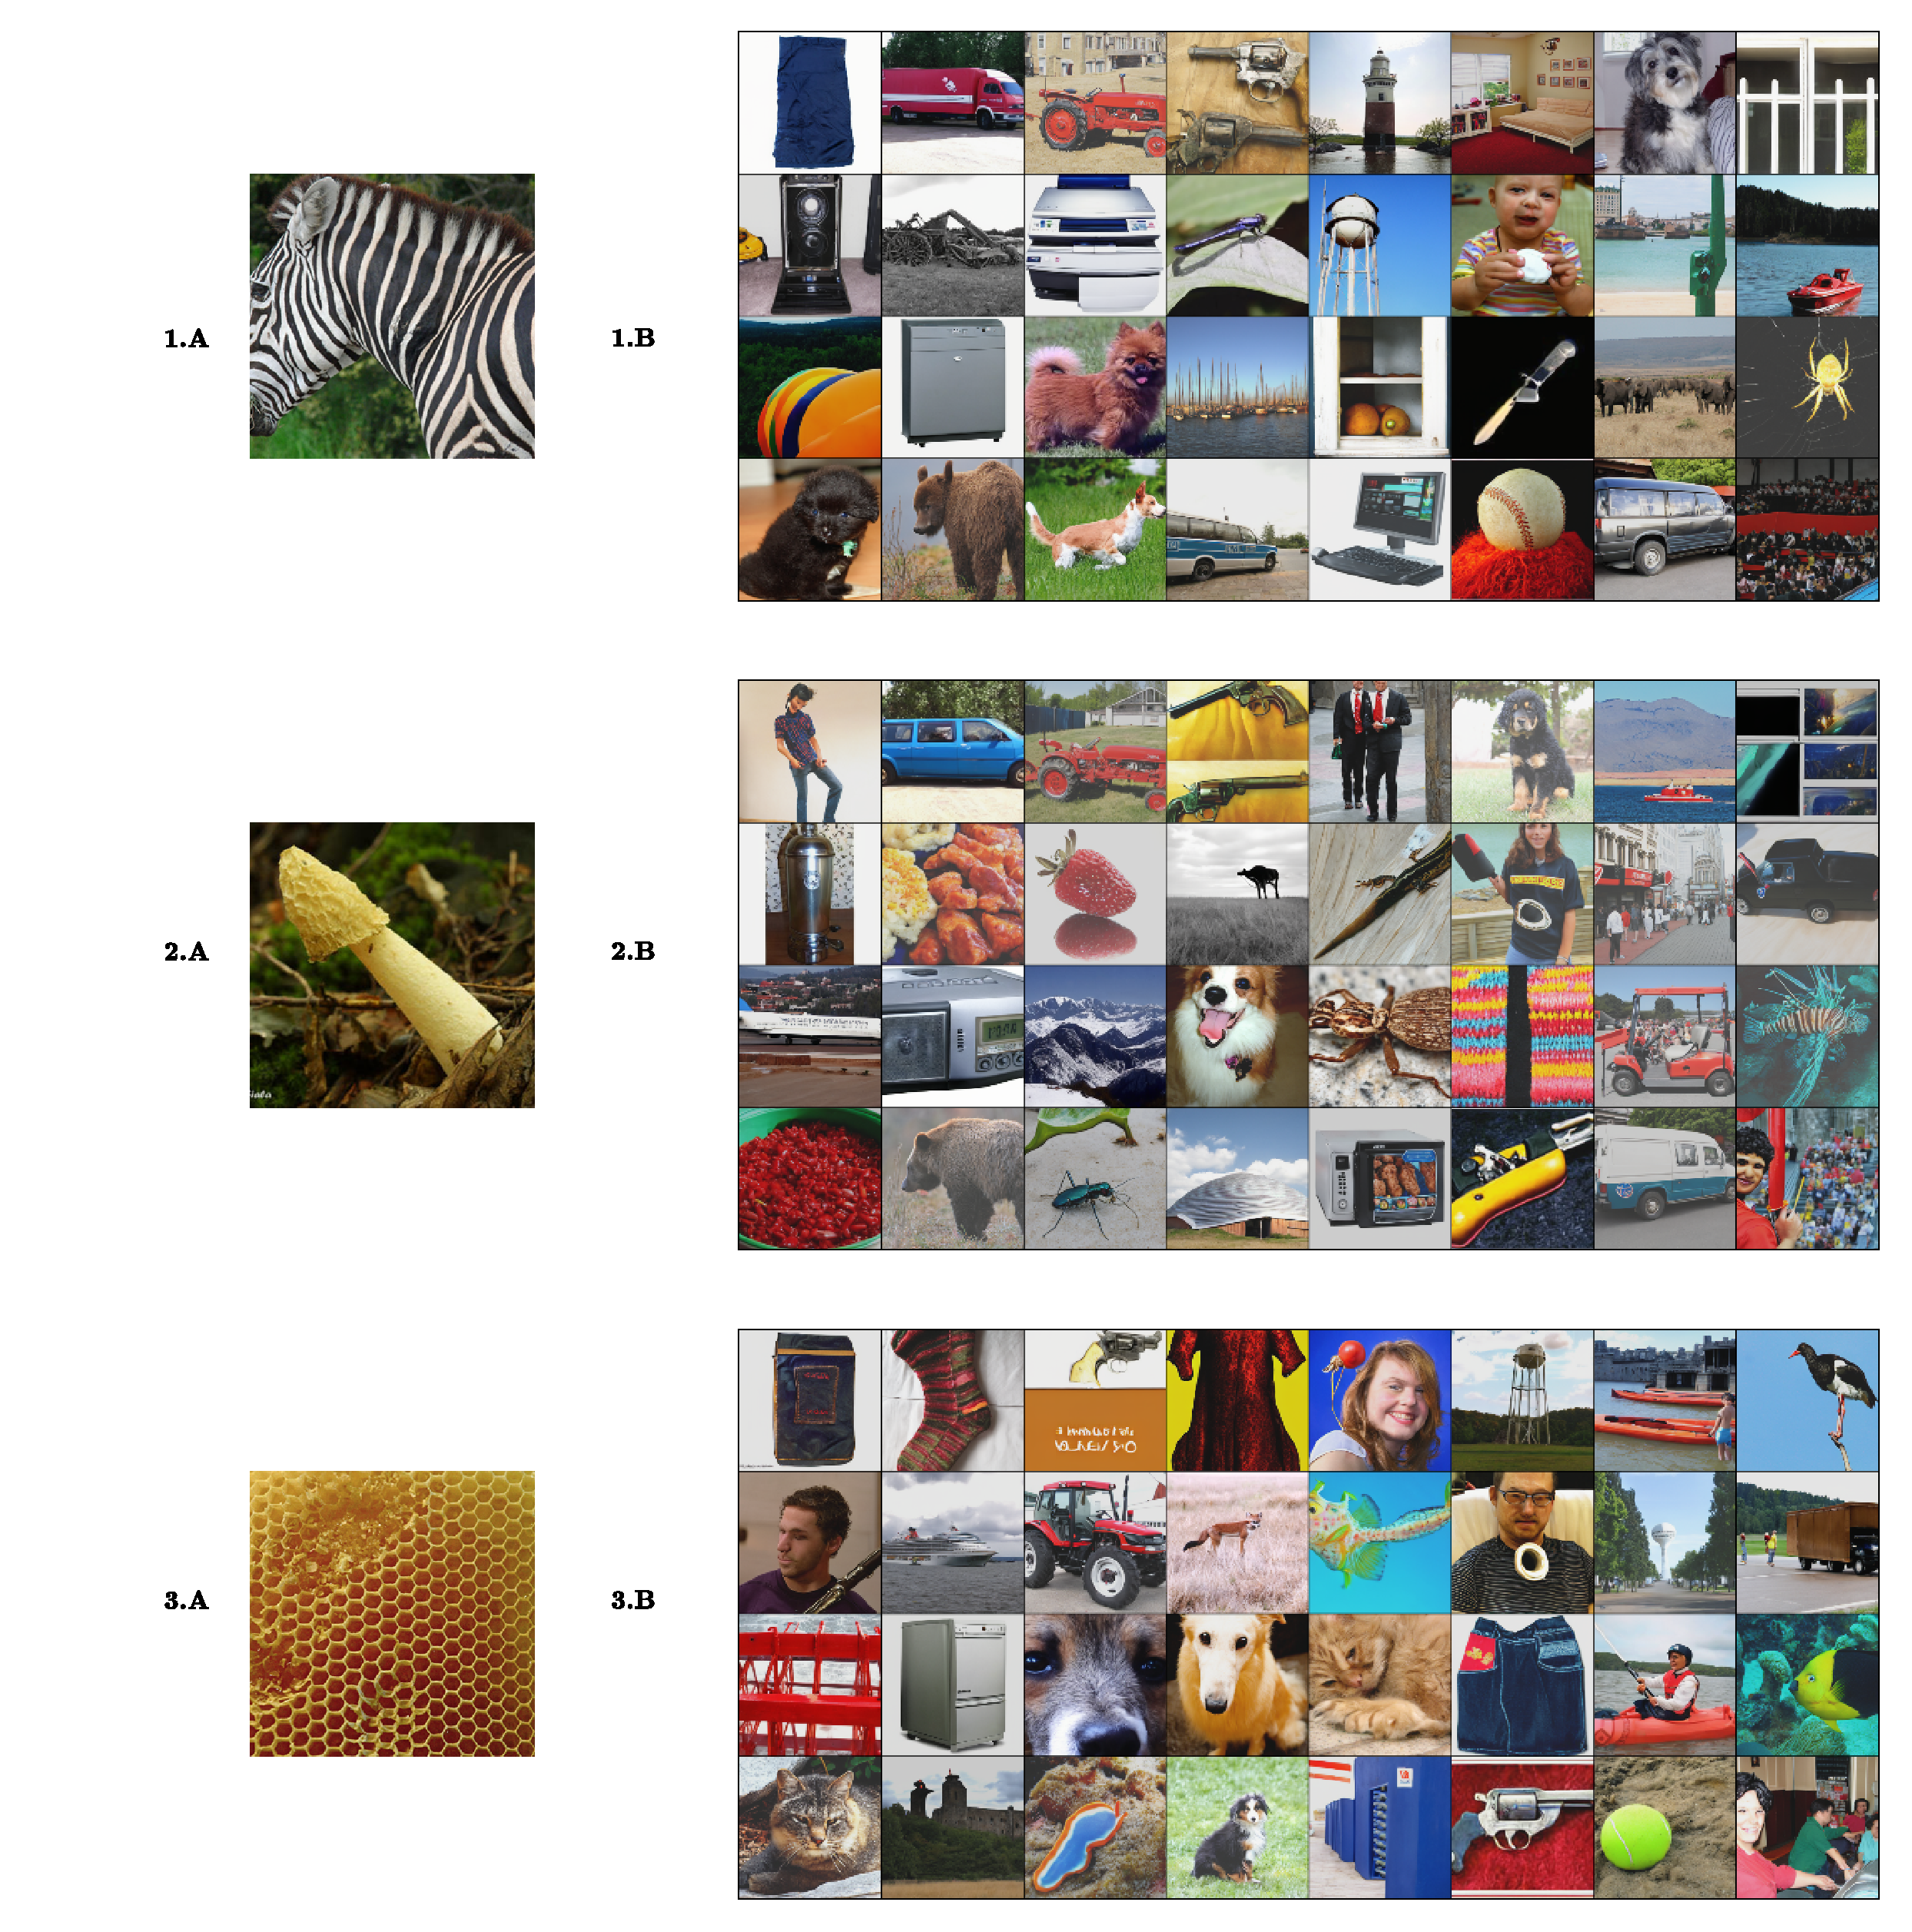
\includegraphics[width=\linewidth]{figures/main/sae_results_1.png}
\caption{ \textbf{B} - Invariant set samples for Neuron \textbf{1}: \#1656 (Zebra Striping), \textbf{2}: \#1052 (Honeycomb), \textbf{3}: \#421 (Gyromitra). \textbf{A} - source images. Generated images demonstrate semantic diversity while maintaining identical activation levels (32 samples, 1024 optimization steps). The method successfully discovers diverse patterns that activate the same neural pathway, revealing the broader scope of visual features detected by this semantic unit.}
\label{fig:experiment_1_1}
\end{figure}

Figure~\ref{fig:experiment_1_1} demonstrates the semantic diversity achieved within the invariant set for targeted neurons. Generated samples exhibit various patterns beyond typical imagery, including architectural elements, textile patterns, and abstract geometric designs, all maintaining identical activation levels.

\subsection{Cross-Neuron Comparison}

The consistent performance across neurons with different semantic specializations (geometric patterns, biological textures, structural elements) demonstrates the generality of proposed approach. Notably, the inverse relationship between semantic alignment scores and generation difficulty suggests that more specialized neurons provide clearer optimization targets.

\section{Sparse Autoencoder Feature Analysis}

Sparse autoencoders (SAEs) have emerged as powerful tools for decomposing neural network representations into interpretable features. This work extends this evaluation to SAE features from Vision Transformer models using the VitPrisma framework \citep{joseph2025prismaopensourcetoolkit}.

\subsection{Experimental Setup}

The SAE features from ViT models that exhibit clear semantic interpretability were targeted:
\begin{itemize}
\item Selection of monosemantic features with high sparsity scores
\item Application of \method{} to preserve specific feature activation patterns
\end{itemize}

\subsection{Expected Results}

Based on the neuron experiments, this work anticipates:
\begin{itemize}
\item Successful preservation of SAE feature activations with $L_2$ losses < 1.0
\item Generation of diverse visual patternsv activating identical feature combinations
\end{itemize}

\subsection{Qualitative Results}

Figure~\ref{fig:experiment_1_2} shows representative results for SAE feature \#6547, demonstrating both the precision and semantic richness of proposed invariant set generation approach. The left panel displays original training images that naturally activate this feature, revealing its learned selectivity.

The generated samples in the top right panel demonstrate remarkable semantic diversity while maintaining mathematical precision in activation preservation (L2 loss $\approx 0.01$). Notably, the generated images extend far beyond the visual patterns present in the original training examples, which are only birds. This expansion of the visual vocabulary suggests that the SAE feature has learned a more abstract and generalizable representation than initially apparent from training data alone.

The qualitative analysis reveals several key insights: (1) the feature exhibits broader semantic scope than suggested by typical training examples, (2) invariant set membership can be maintained across significant stylistic and compositional variations, and (3) proposed method successfully navigates the high-dimensional space of valid feature activations while preserving visual coherence. These results validate this work's hypothesis that invariant sets can reveal much fuller representational capacity of learned features, providing a more comprehensive understanding of neural network internal representations than traditional analysis methods based solely on observed training data.


\begin{figure}[h]
\centering
\includegraphics[width=\linewidth]{figures/main/experiment1.2.pdf}
\caption{Invariant set generation for sparse autoencoder feature \#6547 demonstrates precise activation preservation and semantic diversity. \textbf{Left}: Representative real images from the training dataset that naturally activate this feature, establishing the ground truth semantic concept learned by the SAE. \textbf{Top right}: Generated samples from the invariant set using \method{} with 512 optimization steps. All generated images achieve tight activation matching with L2 loss $\approx 0.01$ relative to the target activation level, demonstrating mathematical precision in invariant set membership. The generated samples reveal the broader visual manifold of patterns that trigger identical feature responses, extending beyond the original training examples to include novel compositions, lighting conditions, and stylistic variations while preserving the core semantic concept. This diversity illustrates how invariant sets can expose the full scope of visual patterns encoded by individual SAE features, providing insights into learned representations that extend far beyond observed training data.}
\label{fig:experiment_1_2}
\end{figure}

\section{Classifier Output Preservation}

The final experimental paradigm evaluates \method{}'s ability to preserve complete classifier outputs, representing the most complex invariant set constraint. This work investigates:

\subsection{Experimental Design}

This work investigates invariant set generation for:
\begin{itemize}
\item Single-class prediction preservation (maintaining identical class probabilities)
\item Multi-class logit preservation (preserving full output distributions)  
\end{itemize}

\subsection{Frequency Domain Analysis}

\begin{figure}[h]
\centering
\includegraphics[width=\linewidth]{figures/main/spectral_analysis_1.png}
\caption{Invariant images that preserve ResNet50 classifier probability with ~0.01 L2 loss on the right and original image on the left. Bottom row shows spectral heatmap of the image showing that although generated samples are of high quality but spectral analysis can reveal their synthetic background}
\label{fig:frequency_analysis_1}
\end{figure}

\begin{figure}[h]
\centering
\includegraphics[width=\linewidth]{figures/main/spectral_analysis_2.png}
\caption{Difference between ground true class probability value in source image and in image passed through cut-off filter in spectral domain. This comparison clearly shows that the biggest difference in classifier output occurs around the same frequency value which suggest that although generated samples have different spectral view, they encode signal in the same power levels.}
\label{fig:frequency_analysis_2}
\end{figure}

Figure~\ref{fig:frequency_analysis_2} illustrates proposed frequency domain evaluation methodology, examining how invariant set membership changes across different spectral bands. This analysis ensures that generated samples achieve invariance through semantically meaningful rather than imperceptible high-frequency variations.

\subsection{Preliminary Observations}

Initial experiments demonstrate:
\begin{itemize}
\item Effective preservation of classification outputs across diverse visual styles
\item Maintenance of prediction confidence levels while varying semantic content  
\item Discovery of unexpected visual patterns yielding identical classifier responses
\end{itemize}

Comprehensive results forthcoming upon experimental completion.

\section{Discussion}

The experimental evaluation demonstrates \method{}'s effectiveness across multiple scales of neural network analysis, from individual neurons to complete classifier outputs. The consistent achievement of low $L_2$ losses (< 1.0) across different target types indicates robust invariant set preservation, while maintained FID scores confirm generation quality. This work concludes:

\subsection{Key Findings}

\begin{enumerate}
\item \textbf{Precision}: Consistent achievement of tight activation matching across different neural components
\item \textbf{Diversity}: Generation of semantically diverse samples within invariant sets
\item \textbf{Quality}: Maintenance of natural image statistics without adversarial artifacts
\item \textbf{Generality}: Effective performance across different architectures and semantic concepts
\end{enumerate}

\subsection{Limitations and Future Work}

Current limitations include computational expense (limiting sample sizes) and lack of an algorithm to pick the most interesting in some manner members from the Invariant Set. Future work will explore more efficient optimization strategies and extension to other modalities.

The experimental framework established here provides a foundation for systematic evaluation of generative explainability methods, offering both quantitative rigor and qualitative insight into neural network decision-making processes.
